\documentclass[10pt,a4paper]{scrartcl}
\usepackage[utf8]{inputenc}
\usepackage{amsmath}
\usepackage{amsfonts}
\usepackage{pgfpages}
\usepackage{amssymb}
\author{Leonard Hackel, Jochen Jacobs, Niklas Schelten}
\title{Manual zur Benutzung des 3D-Druckers}
\begin{document}
\maketitle
\pagebreak
\tableofcontents
\pagebreak
%---------------------------Jochen----------------------------------------------
\section{Erstellen von 3D Objekten}

%---------------------------Hackelle----------------------------------------------
\section{Der Druck}
\begin{center}
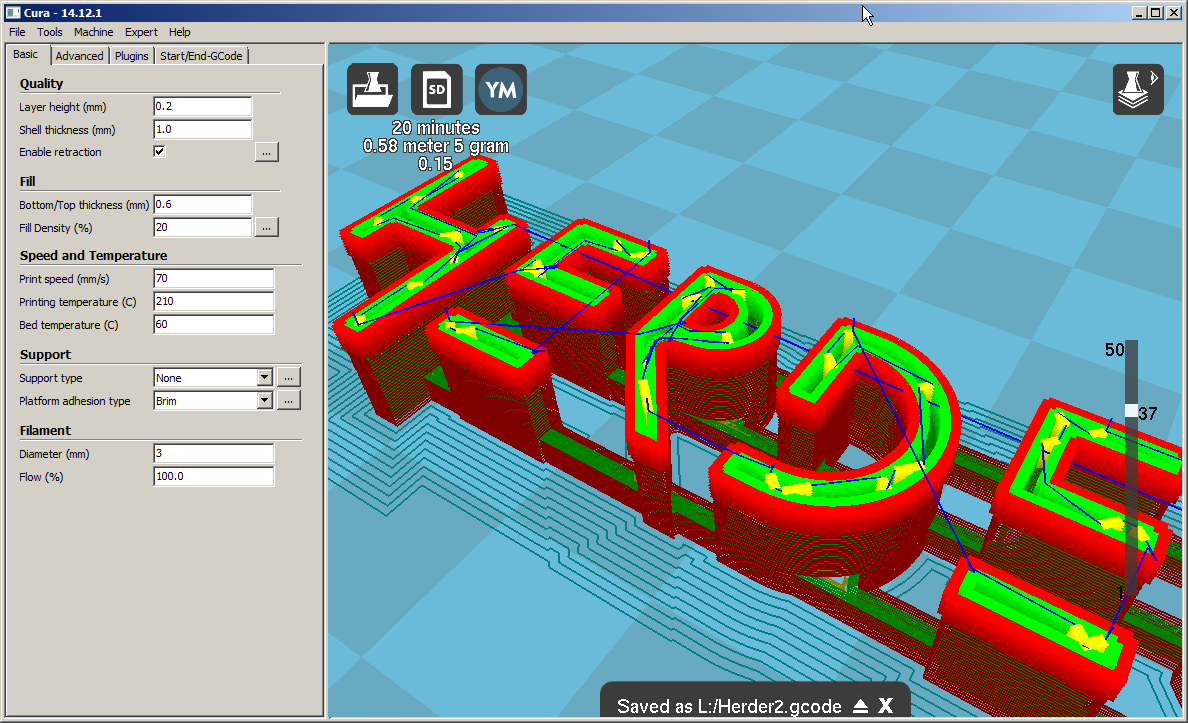
\includegraphics[scale=0.3]{res/Cura-window.png}
\end{center}

Um in diese Ansicht zu gelangen, muss man bei Cura im Reiter "Expert" unter "Switch to full settings" (bzw. "Experte" und "Wechseln zu Expertenmodus") die Ansicht ändern. Dabei verschwinden die Schnelleinstellungen und diese Ansicht erscheint. Das hat den Vorteil, dass die Einstellungen viel genauer vorgenommen werden können.
Das Vorschaufenster bei Cura besteht aus zwei großen Teilen. Auf der linken Seite sind die Einstellungen, auf der rechten ist eine 3D-Ansicht des Objektes. Dabei sind verschiedene Strecken in verschiedenen Farben angezeigt. Innenstrecken sind dabei grün, Druckstrecken, die später Außenflächen ergeben, sind rot, und Strecken, welche der Druckkopf zurücklegt, dabei aber nicht druckt, sind dünner und blau. In gelb dargestellt sind diejenigen Strecken, die später Füllung sind.

%---------------------------Niklas----------------------------------------------
\section{Probleme beim Drucken}
\end{document}